We now introduce our system, called Text2KB\footnote{http://ir.mathcs.emory.edu/projects/text2kb/}, that expands upon the basic KBQA model by incorporating external textual sources throughout the QA process. The general architecture and an example use case of Text2KB is presented on Figure \ref{fig:model}. 
The left part of the figure roughly corresponds to the architecture of existing information extraction approaches to KBQA.
The right part introduces additional external text data sources, specifically
we investigate the use of web search results, community question answering (CQA) data, and a collection of documents with detected KB entity mentions.
We demonstrate how these data sources can help with the main challenges in KBQA, \ie question topical entity identification, predicate scoring and answer candidates ranking.
% Recall that the main challenges in KBQA are linking topical entities in the question to the KB; identifying candidate answers in the neighborhood around the question entities; and ranking the candidates. In the rest of this section we present our approach to solving each of these challenges, by: using web search results, CQA data, and external corpus statistics. 


\subsection{Web search results for KBQA}
\label{section:method:web}

Traditional Text-QA systems rely on search results to retrieve relevant documents, which are then used to extract answers to users' questions.
Relevant search results mention question entities multiple times and in various forms, which can be helpful for question topical entity identification \cite{SMAPH_ERD:2014}.
Furthermore, retrieved document set often contains multiple statements of the answer, which can be a strong signal for candidate ranking \cite{Lin:2007:EPU:1229179.1229180}.

To obtain related web search results, Text2KB issues the question as a query to a commercial web search engine\footnote{https://datamarket.azure.com/dataset/bing/search}, extracts top 10 result snippets and the corresponding documents.
Next, it detects KB entity mentions in both snippets and documents using the same method it applies to the question itself.

\textbf{Question entity identification}.
Question text provides only a limited context for entity disambiguation and linking; additionally, the entity name can be misspelled or an uncommon variation used.
This complicates the task of entity identification, which is the foundation of whole question answering process.
Fortunately, web search results help with these problems, as they usually contain multiple mentions of the same entities and provide more context for disambiguation.
Text2KB uses the search result snippets to \textit{expand} the set of detected question entities.
More specifically, we count the frequencies of each entity mentioned in search snippets, and most popular ones with names similar to some of the question terms are added to the list of topical entities.
The goal of this similarity condition is to keep only entities that are likely mentioned in the question text and filter out simply related entities.
To estimate the similarity between a name and question tokens we use Jaro-Winkler string distance, an entity is added to the list of question entities if at least one of its tokens $e_t$ has high similarity with one of the question tokens $q_t$ excluding stopwords ($Stop$):
$$\max_{e_t \in M\backslash Stop, q_t \in Q\backslash Stop} 1 - dist(e_t, q_t) \geq 0.8$$

\textbf{Answer candidate features}.
The information stored in KBs can also be present in other formats, \eg text statements.
For example, on Figure \ref{fig:web_search_entitylink} multiple snippets mention the date when Tutankhamun became the king.
Text-QA systems use such passages to extract answer to users' questions.
However, text provides very little context information about the mentioned entities, and systems have to infer the useful details, \eg entity types, which can be problematic \cite{yih2015semantic}.
On the other hand, KBQA systems can utilize all the available KB knowledge about the entities in a candidate answer, and would benefit from additional text-based information to improve ranking.
More specifically, we perform the following:

\begin{enumerate}[noitemsep,topsep=0pt]
\item Precompute term and entity IDFs. We used Google n-grams corpus to approximate terms IDF by collection frequencies and available ClueWeb Freebase entity annotations\footnote{http://lemurproject.org/clueweb09/FACC1/} to compute entity IDFs
\item Each snippet and document is represented by two TF-IDF vectors of lowercased tokens and mentioned entities
\item In addition, vectors of all snippets and all documents are merged together to form combined token and entity vectors
\item Each answer candidate is also represented as TF-IDF vectors of terms (from entity names) and entities
\item We compute cosine similarities between answer and each snippet and document token and entity vectors. This gives us 10 similarity scores for every document for token vectors and 10 similarities for entity vectors. We take average and maximum scores as features.
\item We do the same for the combined document and use cosine similarities as features.
\end{enumerate}

\subsection{CQA data for Matching Questions to Predicates}
\label{section:method:cqa}

Recall that a major challenge in KBQA is that natural language questions do not easily or uniquely map to entities and predicates in a KB.
An established approach for this task is supervised machine learning, which requires labeled examples of questions and the corresponding answer to learn this mapping, which can be expensive.
% On the other hand, there are huge archives of questions and answers posted by real users on various community question answering websites, \eg Figure \ref{fig:cqa_example}.
% Unfortunately, manual labeling of questions with answers is expensive, and necessarily contains only a small fraction of the different ways the same KB predicate can be inquired about using natural language questions.
Researchers have proposed to use weakly supervised methods to extend a lexicon with mappings learned from \textit{single sentence statements} mentioning entity pairs in a large corpus \cite{yao2014information}.
However, the language used in questions to query about a certain predicate may differ from the language used in statements.
A recent work~\cite{savenkov-EtAl:2015:SRW} demonstrated how distant supervision assumption can be applied to question-answer pairs from CQA archives for a related task of information extraction for knowledge base completion.
In a similar way, we use weakly labeled collection of question-answer pairs to compute associations between question terms and predicates to \textit{extend} system's lexicon (Figure \ref{fig:cqa_example}).
We should emphasize, that this data doesn't replace the mappings, learned from single sentence statements, which are already used by our baseline systems, but rather extend it.
Weakly labeled question-answer pairs are usually more noisy than sentences, but can provide complementary information \cite{savenkov-EtAl:2015:SRW}.

\begin{figure}
\centering
\fbox{
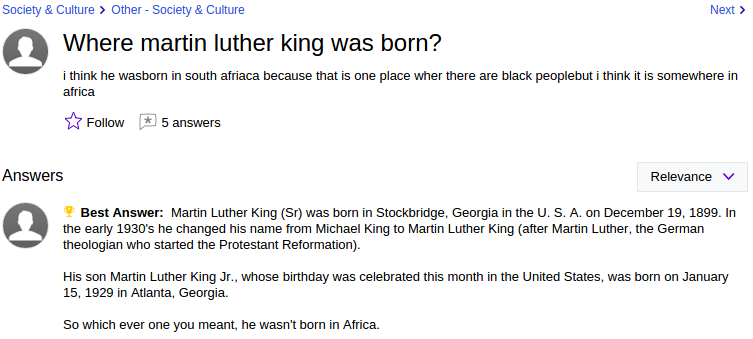
\includegraphics[width=0.4\textwidth]{img/cqa_example}
}
\vspace{-3mm}
\caption{Example of a question and answer pair from Yahoo! Answers CQA website}
\label{fig:cqa_example}
\end{figure}

For our experiments we use 4.4M questions from Yahoo! WebScore L6 dataset\footnote{https://webscope.sandbox.yahoo.com/catalog.php?datatype=l}.
Question and answer texts were run through an entity linker, that detected mentions of Freebase entities.
Next, we use distant supervision assumption to label each question-answer pair with predicates between entities mentioned in the question and in the answer.
% As a result, we have a set of questions, annotated with KB predicates, which are, often incorrectly, assumed to answer the question.
This labels are used to learn associations between question terms and predicates by computing pointwise mutual information scores (PMI) for each term-predicate pair.
Examples of scores for some terms are given in Table \ref{table:cqa_npmi}.

\begin{table}
\begin{tabular}{| p{1cm} | p{5.5cm} | p{0.75cm} |}
\hline
Term & Predicate & PMI score\\
\hline
born & people.person.date\_of\_birth & 3.67\\
 & people.person.date\_of\_death & 2.73\\
 & location.location.people\_born\_here & 1.60\\
\hline
kill & people.deceased\_person.cause\_of\_death & 1.70\\
& book.book.characters & 1.55\\
\hline
currency & location.country.currency\_formerly\_used & 5.55 \\
& location.country.currency\_used & 3.54 \\
\hline
school & education.school.school\_district & 4.14 \\
& people.education.institution & 1.70\\
& sports.school\_sports\_team.school & 1.69 \\
%\hline
%illness & medicine.symptom.symptom\_of & 2.11\\
%& medicine.decease.causes & 1.68\\
%& medicine.disease.treatments & 1.59\\
\hline
win & sports.sports\_team.championships & 4.11\\
& sports.sports\_league.championship & 3.79\\
\hline
\end{tabular}
\vspace{-3mm}
\caption{Examples of term-predicate pairs with high PMI scores, computed using distant supervision from a CQA collection}
\label{table:cqa_npmi}
\end{table}

In Text2KB we take candidate answer predicates and look up the PMI scores between them and terms in the question (missing pairs are given a score of 0).
From this list of score we compute minimum, average and maximum and add these values to the feature list.
Since this kind of data is usually sparse, we also use pretrained word2vec word embeddings\footnote{https://code.google.com/p/word2vec/}.
We compute predicate embeddings by taking a weighted average of term vectors from predicate's PMI table.
Each term vector is weighted by its PMI value (terms with negative score are skipped).
Then, we compute cosine similarities between predicate vector and each of the question term vectors and take their minimum, average, maximum as features.
Finally, we average embeddings of question terms and compute its cosine similarity with the predicate vector.

\subsection{Estimating Entity Associations}
\label{section:method:clueweb}

A key step for ranking candidate answers is to estimate whether the question and answer entities are related in a way asked in the question.
Existing KBQA approaches usually focus on scoring the mappings between question phrases and KB concepts from a candidate SPARQL query.
However, textual data can provide another angle on the problem, as question and answer entities are likely to be mentioned together somewhere in text passages.
For example, in the bottom right corner of Figure \ref{fig:model} we can see some passages that mention a pair of people, and the context of these mentions explains the nature of the relationships.
This data can be viewed as additional edges in a KB, that connect pairs of entities, and have associated language models, estimated from text phrases, that mention these entities.
Such edges do not have to coincide with the existing KB edges, and can connect arbitrary pairs of entities, that are mentioned together in text, therefore extending the KB.

We use the ClueWeb12 corpus with existing Freebase entity annotations and count different terms that occur in the context of a mention of a pair of different entities (we only consider mentions within 200 characters of each other).
To compute this unigram language model we take terms in between and 100 character before and after entity mentions.
A small sample of this data is presented in Table \ref{table:clueweb_entitypairs_langmodel}.

\begin{table}
\begin{tabular}{| p{1.25cm} | p{1.23cm} | p{4.5cm} |}
\hline
Entity 1 & Entity 2 & Term counts\\
\hline
John Edwards & Rielle Hunter & campaign, affair, mistress, child, former ...\\
\hline
John Edwards & Cate Edwards & daughter, former, senator, courthouse, greensboro, eldest ...\\
\hline
John Edwards & Elizabeth Edwards & wife, hunter, campaign, affair, cancer, rielle, husband ...\\
\hline
John Edwards & Frances Quinn & daughter, john, rielle, father, child, former, paternity...\\
\hline
\end{tabular}
\vspace{-2mm}
\caption{Example of entity pairs along with the most popular terms mentioned around the entities}
\label{table:clueweb_entitypairs_langmodel}
\end{table}

We use this data to compute candidate ranking features in the following way.
Let us have question words $Q$ and an answer candidate, which contains a question entity $e_1$ and one or more answer entities $e_2$.
For each answer we compute a language model score:
$$p(Q|e_1, e_2) = \prod_{t\in Q} p(t | e_1, e_2)$$
and use minimum, average and maximum over all answer entities as features.
To address the sparsity problem, we again use embeddings, 
\ie for each entity pair a weighted (by counts) average embedding vector of terms is computed and minimum, average and maximum cosine similarities between these vectors and question token embeddings are used as features.

\subsection{Internal text data to enrich entity representation}
In addition to external text data, many knowledge bases, including Freebase, contain text data as well, \eg Freebase includes a description paragraph from Wikipedia for many of its entities.
These text fragments provide a general description of entities, which may include information relevant to the question, which was found useful for Text-QA \cite{Sun:2015:ODQ:2736277.2741651}.
For completeness, we include them in our system as well.
Each entity description is represented by a vector of tokens, and a vector of mentioned entities.
We compute cosine similarities between token and entity vectors of the question and description of each of the answer, and use minimum, average and maximum of the scores as features.
% In future work, we could explore incorporating any other entity profile text, such as full Wikipedia article.
